% book_example.tex - Test for Book Class Support (v7.0.4)
% This example demonstrates all book-specific features of hebrew-academic-template
% Compiler: LuaLaTeX
%
% Features demonstrated:
%   - Book class with frontmatter/mainmatter/backmatter
%   - hebrewchapter, hebrewappendix commands
%   - 'definition', 'abstract' environments
%   - TOC BiDi fixes (page numbers LTR, dot leaders)
%   - Modern tabularray tables with fancytable
%   - Code blocks with pythonbox
%   - Cross-chapter references

\documentclass[book]{hebrew-academic-template}

\addbibresource{example_references.bib}

\begin{document}

%% ============================================
%% Front Matter
%% ============================================
\frontmatter

%% Title Page
\begin{titlepage}
\begin{center}
\vspace*{2cm}
{\Huge\bfseries ספר בדיקה לתבנית}
\vspace{0.5cm}

{\Large\en{Test Book for Hebrew Academic Template}}
\vspace{1cm}

{\large הדגמת תכונות התבנית האקדמית העברית}
\vspace{2cm}

{\Large מאת}
\vspace{0.5cm}

{\Large\bfseries דר' יורם סגל}
\vspace{3cm}

{\large גרסת \en{CLS}: \en{\clsversion}}
\vspace{2cm}

{\normalsize מהדורה ראשונה -- דצמבר \en{2025}}
\end{center}
\end{titlepage}

%% Copyright Page
\newpage
\thispagestyle{empty}
\vspace*{\fill}
\begin{center}
{\small כל הזכויות שמורות \textenglish{©} \en{2025}}
\end{center}
\vspace*{\fill}

%% Abstract
\newpage
\begin{abstract}
ספר זה מהווה מדריך מקיף לתבנית האקדמית העברית גרסה \en{\clsversion}. התבנית תומכת בכתיבה דו-כיוונית (\en{BiDi}) עבור מסמכים אקדמיים הכוללים עברית ואנגלית.

התבנית כוללת תמיכה מלאה במחלקת ספר (\en{book class}):
\begin{itemize}
    \item מבנה ספר מלא עם \en{frontmatter/mainmatter/backmatter}
    \item תוכן עניינים, רשימת איורים, ורשימת טבלאות בעברית
    \item פרקים עבריים עם מספור \en{LTR}
    \item נספחים עם מספור עברי (א, ב, ג)
    \item סביבות מעוצבות: \en{definition}, \en{abstract}, \en{notebox}, \en{warningbox}
    \item טבלאות מודרניות עם \en{tabularray} וערכות נושא מובנות
\end{itemize}
\end{abstract}

%% Table of Contents
\tableofcontents

%% List of Figures
\listoffigures

%% List of Tables
\listoftables

%% Preface
\chapter*{הקדמה}
\addcontentsline{toc}{chapter}{הקדמה}

זהו ספר להדגמת תכונות מחלקת הספר (\en{book class}) בתבנית האקדמית העברית גרסה \en{\clsversion}.
התבנית מבוססת על עקרונות מודרניים של עיבוד שפה טבעית \cite{vaswani2017attention}.

\hebrewsection{תכונות עיקריות}

\begin{itemize}
    \item \textbf{מבנה ספר}: תמיכת מחלקת ספר (\en{book class})
    \begin{itemize}
        \item \en{frontmatter/mainmatter/backmatter}
        \item \en{\textbackslash hebrewchapter\{\}} ו-\en{\textbackslash hebrewappendix\{\}}
        \item תוכן עניינים, רשימת איורים, רשימת טבלאות בעברית
    \end{itemize}

    \item \textbf{סביבות מעוצבות}:
    \begin{itemize}
        \item סביבת \en{abstract} למצב ספר
        \item סביבת \en{definition} לתיבות הגדרה
        \item \en{notebox}, \en{warningbox}, \en{examplebox}
    \end{itemize}

    \item \textbf{טבלאות מודרניות}:
    \begin{itemize}
        \item \en{fancytable} -- טבלה פשוטה עם כותרת
        \item ארבע ערכות נושא: \en{fancy}, \en{minimal}, \en{striped}, \en{academic}
        \item יישור עברי (\en{RTL}) תקין בכל הטבלאות
    \end{itemize}

    \item \textbf{קוד ותמונות}:
    \begin{itemize}
        \item \en{pythonbox} לקוד \en{Python} עם הדגשת תחביר
        \item תמיכה בתמונות ואיורי \en{TikZ}
    \end{itemize}
\end{itemize}

\hebrewsection{הפניות לפרקים}

ניתן להפנות לפרקים באמצעות \en{\textbackslash ref\{\}}:
\begin{itemize}
    \item פרק~\ref{chap:intro} -- פרק ראשון
    \item פרק~\ref{chap:tables} -- טבלאות ואיורים
    \item פרק~\ref{chap:refs} -- הפניות
\end{itemize}

%% ============================================
%% Main Matter
%% ============================================
\mainmatter

%% Chapter 1
\hebrewchapter{פרק ראשון - מבוא}
\hebrewchapterlabel{chap:intro}

זהו הפרק הראשון בספר הבדיקה. המספור צריך להיות \en{1} ב-\en{LTR}.

\hebrewsection{סעיף ראשון}

סעיף זה צריך להיות ממוספר \en{1.1}.

\begin{notebox}[הערה חשובה]
זוהי תיבת הערה (\en{notebox}) עם תמיכת \en{BiDi}. הרקע לא צריך לגלוש מחוץ לשוליים.
\end{notebox}

\hebrewsubsection{תת-סעיף ראשון}

תת-סעיף זה צריך להיות ממוספר \en{1.1.1}.

\begin{examplebox}[דוגמה]
זוהי תיבת דוגמה (\en{examplebox}) עם תמיכת \en{BiDi}.
\end{examplebox}

\hebrewsubsubsection{תת-תת-סעיף}

תת-תת-סעיף זה צריך להיות ממוספר \en{1.1.1.1}.

%% Definition Environment (v5.11.1 - New styled box)
\begin{definition}[הגדרה מתמטית]
\textbf{תבנית אקדמית} היא מסמך \LaTeX{} המותאם לכתיבה אקדמית בעברית ובאנגלית, עם תמיכה מלאה ב-\en{BiDi} (דו-כיווניות).

נוסחה לדוגמה:
\[
E = mc^2
\]

כאשר \en{E} מייצג אנרגיה, \en{m} מסה, ו-\en{c} מהירות האור.
\end{definition}

\hebrewsection{סעיף שני}

סעיף זה צריך להיות ממוספר \en{1.2}.

\begin{warningbox}[אזהרה]
זוהי תיבת אזהרה (\en{warningbox}) עם תמיכת \en{BiDi}.
\end{warningbox}

%% Chapter 2
\hebrewchapter{פרק שני - טבלאות ואיורים}
\hebrewchapterlabel{chap:tables}

פרק זה מדגים טבלאות ואיורים.

\hebrewsection{טבלה לדוגמה}

\begin{fancytable}{ccc}{טבלת בדיקה}
\label{tab:test}
עמודה א & עמודה ב & עמודה ג \\
ערך \en{1} & ערך \en{2} & ערך \en{3} \\
תוכן & מידע & נתון נוסף \\
\end{fancytable}

\hebrewsection{טבלה עם צבעי שורות}

טבלה זו מדגימה את ערכת הנושא \en{striped} עם שורות מתחלפות:

\begin{table}[H]
\centering
\caption{טבלה עם שורות צבעוניות}
\label{tab:colored}
\begin{tblrstriped}{R{3cm}R{4cm}R{2cm}}
גרסה & תכונה & סטטוס \\
\en{v7.0.0} & תמיכת \en{tabularray} & פעיל \\
\en{v7.0.3} & יישור עברי בטבלאות & פעיל \\
\en{v7.0.4} & תיקון עמודות \en{R\{\}} & פעיל \\
\end{tblrstriped}
\end{table}

\hebrewsection{איור לדוגמה}

\begin{figure}[H]
\centering
\begin{english}
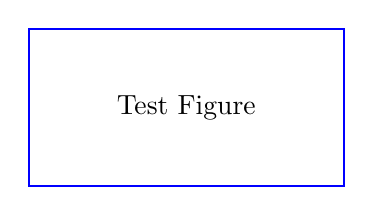
\begin{tikzpicture}
\draw[thick, blue] (0,0) -- (4,0) -- (4,2) -- (0,2) -- cycle;
\node at (2,1) {Test Figure};
\end{tikzpicture}
\end{english}
\caption{איור בדיקה}
\label{fig:test}
\end{figure}

%% Chapter 3
\hebrewchapter{פרק שלישי - הפניות}
\hebrewchapterlabel{chap:refs}

ניתן להפנות לפרק~\ref{chap:intro}, לטבלה~\ref{tab:test}, ולאיור~\ref{fig:test}.

\hebrewsection{קוד לדוגמה}

הקוד הבא מדגים את סביבת \en{pythonbox} עם הדגשת תחביר:

\begin{english}
\begin{pythonbox}[\hebtitle{קוד \en{Python} לדוגמה}]
def hello_world():
    # Function to greet the world
    message = "Hello World with spaces"
    greeting = "Shalom"
    print(f"Message: {message}")
    print(f"Greeting: {greeting}")
    return True

# Test various string patterns
test_strings = [
    "hello world",      # Simple spaces
    "a    b    c",      # Multiple spaces
    "   leading",       # Leading spaces
    "trailing   "       # Trailing spaces
]
\end{pythonbox}
\end{english}

%% ============================================
%% Back Matter
%% ============================================
\backmatter

%% Bibliography (English references - left-aligned, LTR)
\begin{english}
\printbibliography[heading=bibintoc,title={References}]
\end{english}

%% Appendices
\appendix

\hebrewappendix{נספח ראשון}

זהו הנספח הראשון. המספור צריך להיות א (אלף עברי).

\hebrewappendix{נספח שני}

זהו הנספח השני. המספור צריך להיות ב (בית עברי).

\end{document}
